\begin{activity}\label{A:0.2.3}
The quantity, $Q$, of a drug in a patient's body at time $t$ is represented for positive
constants $S$ and $k$ by the function $Q(t) = S(1-e^{-kt})$. 
\ba
\item For $t \ge 0$ describe how $Q(t)$ changes with time.
\item Assuming that $S = 5$, use a graphing utility to make a sketch of $Q(t)$ with
    various values of $k$.  Use the left-hand side of Figure \ref{F:0.2.Act3} to organize
    your plots.  Interpret the value of $k$ in the context of this problem.
\item Now assume that $k=0.5$ and use a graphing utility to make a sketch of $Q(t)$ with
    various values of $S$.  Use the right-hand side of Figure \ref{F:0.2.Act3} to organize
    your plots.  Interpret the value of $S$ in the context of this problem.
\ea
\begin{figure}[h!]
    \begin{center}
        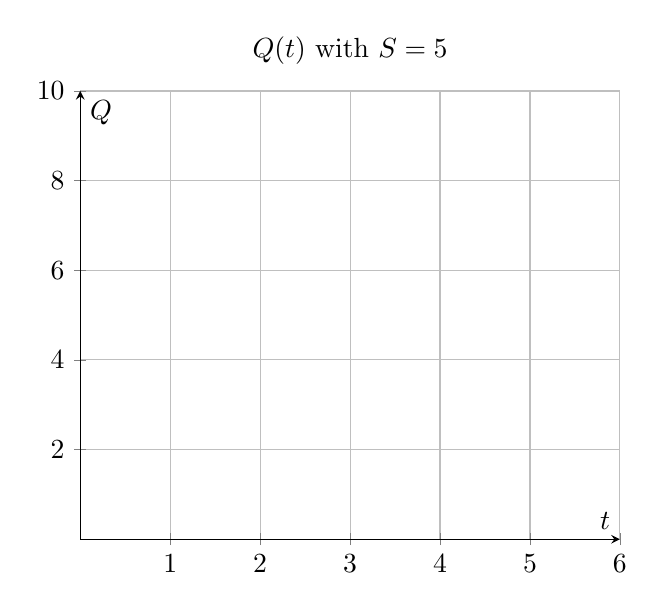
\begin{tikzpicture}
            \begin{axis}[axis lines=center,xlabel={$t$}, ylabel={$Q$}, xmin=0, ymin=0, xmax=6,
                ymax=10, grid, title={$Q(t)$ with $S=5$}]
                \addplot[smooth] {0*x};
            \end{axis}
        \end{tikzpicture}
        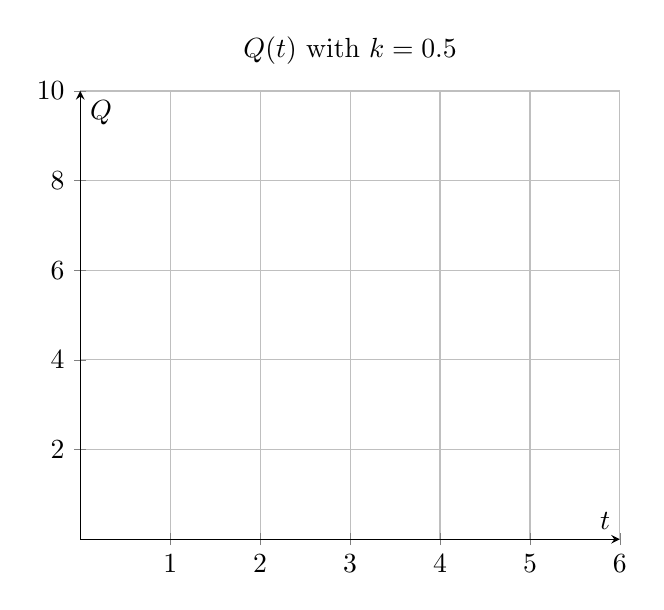
\begin{tikzpicture}
            \begin{axis}[axis lines=center,xlabel={$t$}, ylabel={$Q$}, xmin=0, ymin=0, xmax=6,
                ymax=10, grid, title={$Q(t)$ with $k=0.5$}]
                \addplot[smooth] {0*x};
            \end{axis}
        \end{tikzpicture}
    \end{center}
    \caption{Plot for Activity \ref{A:0.2.3}}
    \label{F:0.2.Act3}
\end{figure}
\end{activity}\aftera
